%%% IMPORTANT: COMPILE WITH XeLaTeX

\documentclass[12pt]{article}
%All packages used this far
%\usepackage[latin1]{inputenc}
%\usepackage{times}
%\usepackage{logicproof}
%\usepackage{enumerate}
%\usepackage{cancel}
\usepackage{fullpage} % required for this template
%\usepackage{color}
%\usepackage{qtree}
%\usepackage{amsmath}
\usepackage{fontspec} % required for this template
%\usepackage{amssymb}
%\usepackage{amsthm}
%\usepackage{prooftrees}
\usepackage{tikz}
%\usepackage{circuitikz}
%\usepackage{colortbl}
%\usepackage{karnaugh-map}
%\usepackage[margin=1in]{geometry} % not sure if useful
%\usepackage{indentfirst}
%\usepackage{pgfplots}
%\usepackage{xcolor}
%\usepackage{arydshln}
%\usepackage{hyperref}

% Tikz libraries
%\usetikzlibrary{positioning}
%\usetikzlibrary{shapes.multipart}
%\usetikzlibrary{decorations.text}
%\usetikzlibrary{datavisualization}
%\usetikzlibrary{datavisualization.formats.functions}
%\usetikzlibrary{patterns}
%\usetikzlibrary{arrows.meta}
%\usetikzlibrary{quotes}
%\usetikzlibrary{automata}


\setromanfont{Times New Roman}
\setsansfont{Helvetica}

%Symbols that might be necessary
%\DeclareMathSymbol{@}{\mathord}{letters}{"3B}
%\newcommand{\powerset}{\raisebox{.15\baselineskip}{\Large\ensuremath{\wp}}}

\begin{document}

\noindent
Universidade Federal do Rio Grande do Sul \hfill Instituto de Informática \newline 
INF01009 -- Computação Gráfica \hfill 2023/1 \newline
Aluno \hfill Pedro Company Beck -- 00324055
\rule{\linewidth}{1.pt}

\begin{center}
	\LARGE\textbf{Assignment 3} 
\end{center}

Rasterization was implemented in Close2GL, and it's being done by making color and z buffers, then mapping the color buffer as a texture to two triangles that will be shown on the screen.\\
Each pixel of the color buffer has a \texttt{z} value that is compared for every fragment to check whether it will be visible or not. The implementation can be checked in the source code that will be provided with this report.\\

Close2GL now supports rasterization of a model as points:
\begin{center}
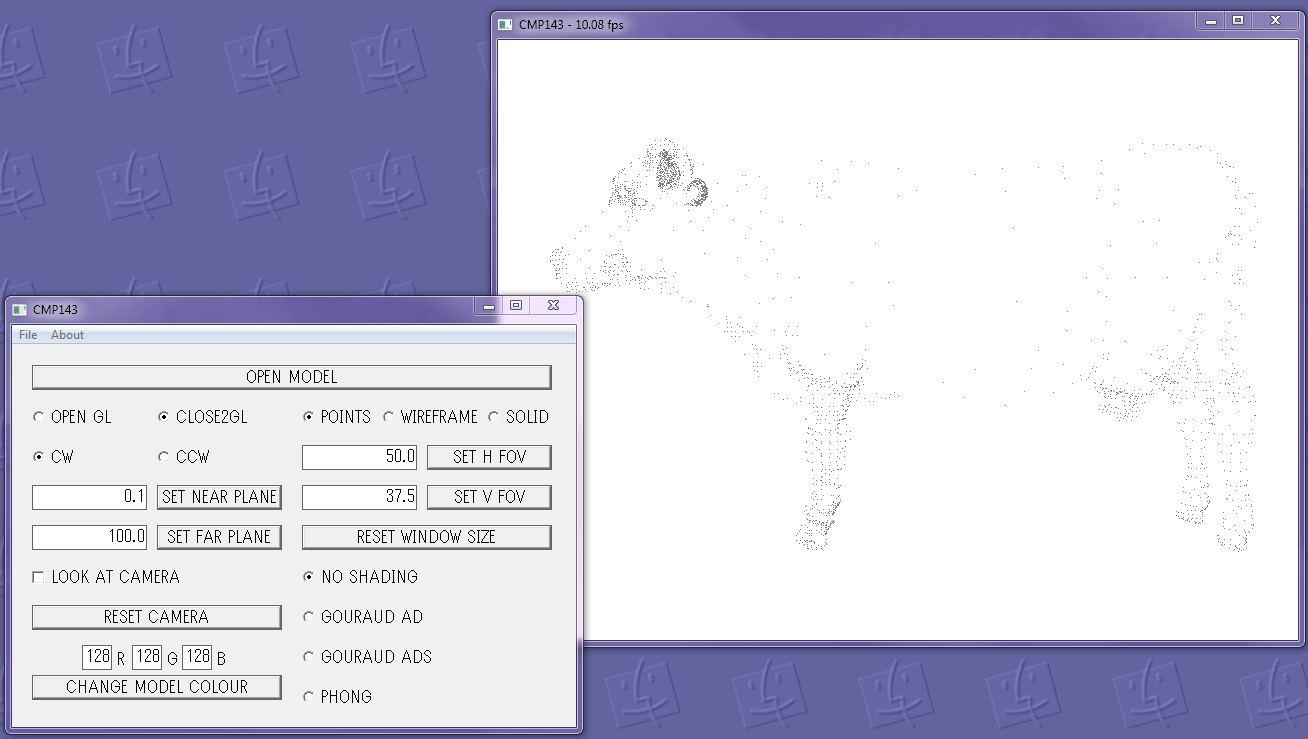
\includegraphics[scale=0.45]{3.png}
\end{center}
\newpage
As wireframe:
\begin{center}
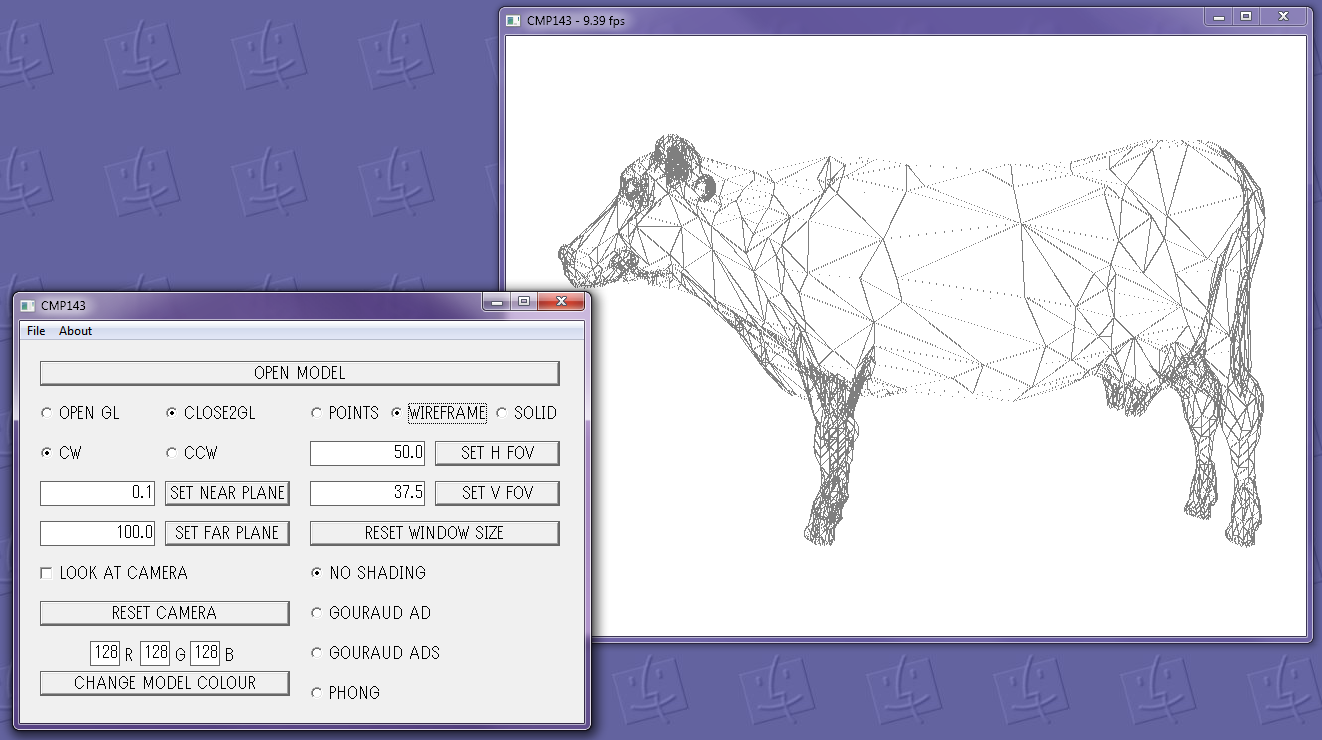
\includegraphics[scale=0.45]{2.png}
\end{center}
unfortunately, some of the edges are not entirely connected as lines, this is due to the rasterization function only printing the first and last pixels of the row that's being drawn at any moment.
\newpage
And as a solid:
\begin{center}
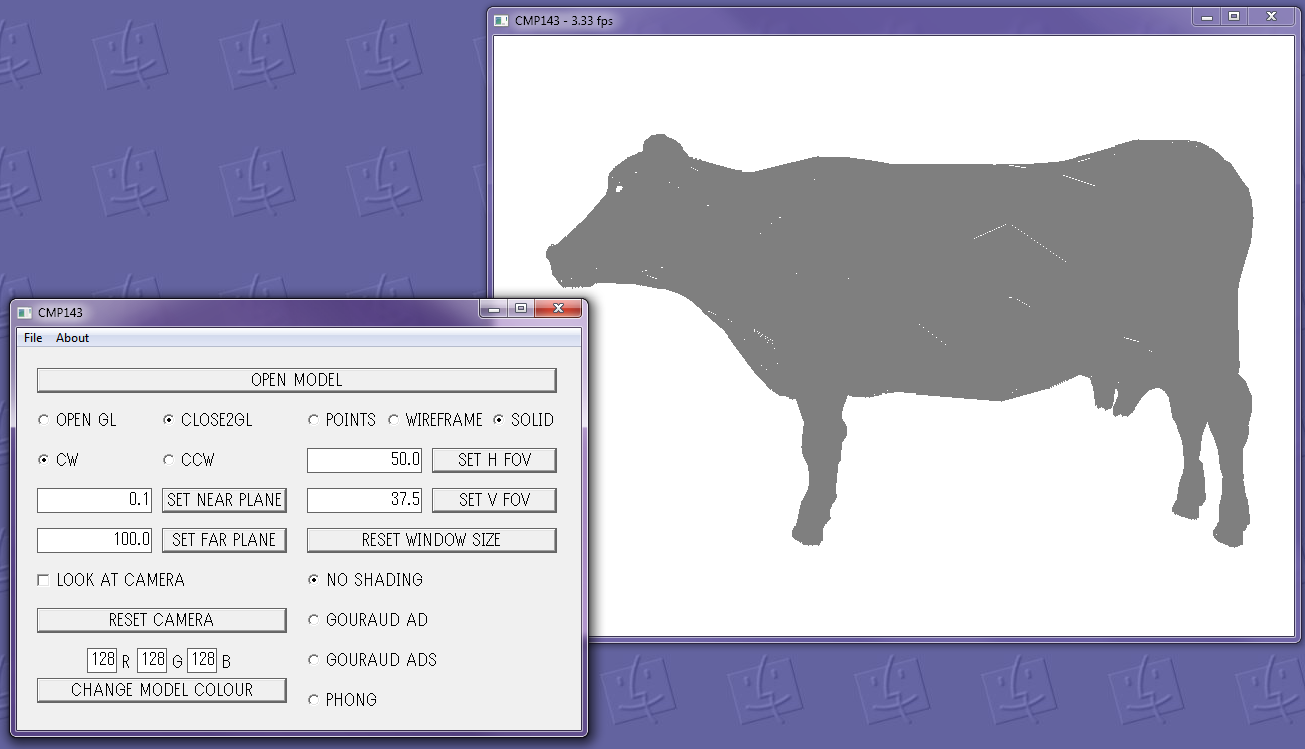
\includegraphics[scale=0.45]{1.png}
\end{center}
unfortunately, there are some visible artifacts. This may have been due to the usage of the \texttt{floor()} function to approximate the pixel values to integers and some tests were made, however, the cause is still unknown.
\newpage
Close2GL also supports rasterization with Gouraud AD and Gouraud ADS (or Phong) lightning models:
\begin{center}
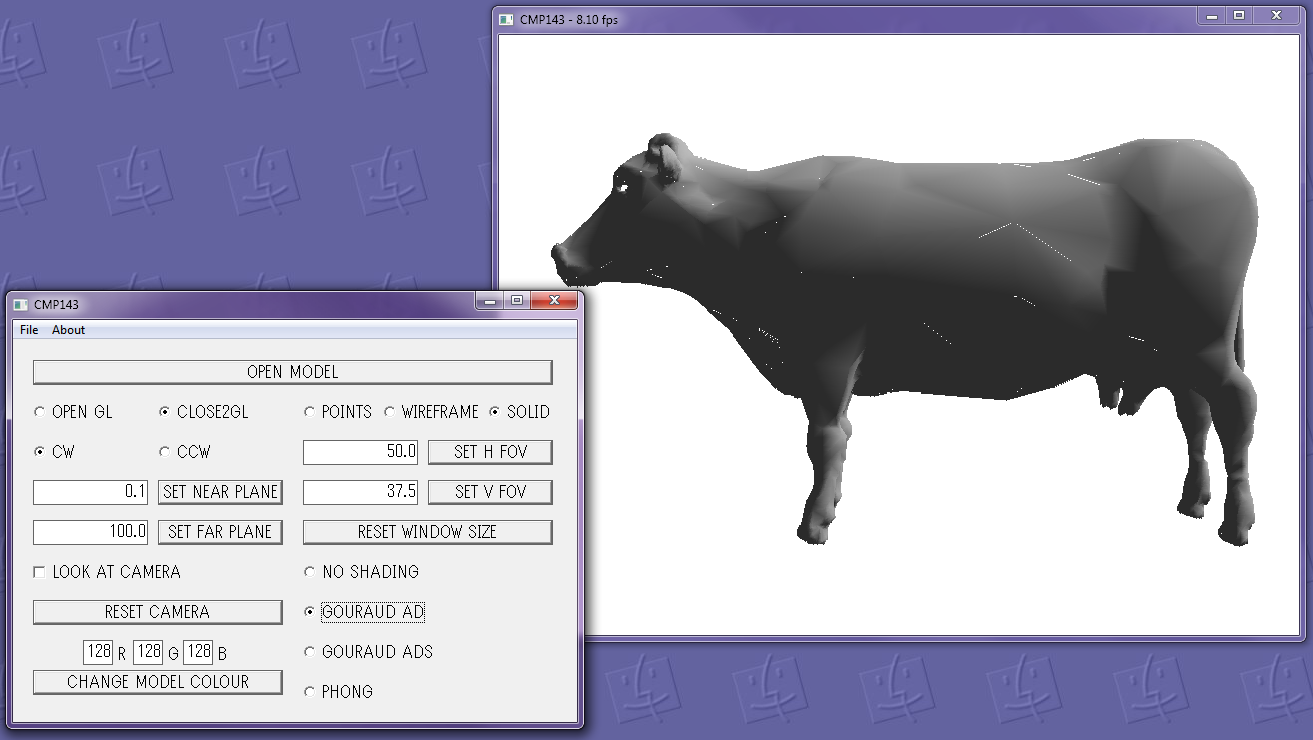
\includegraphics[scale=0.45]{4.png}
\end{center}
\begin{center}
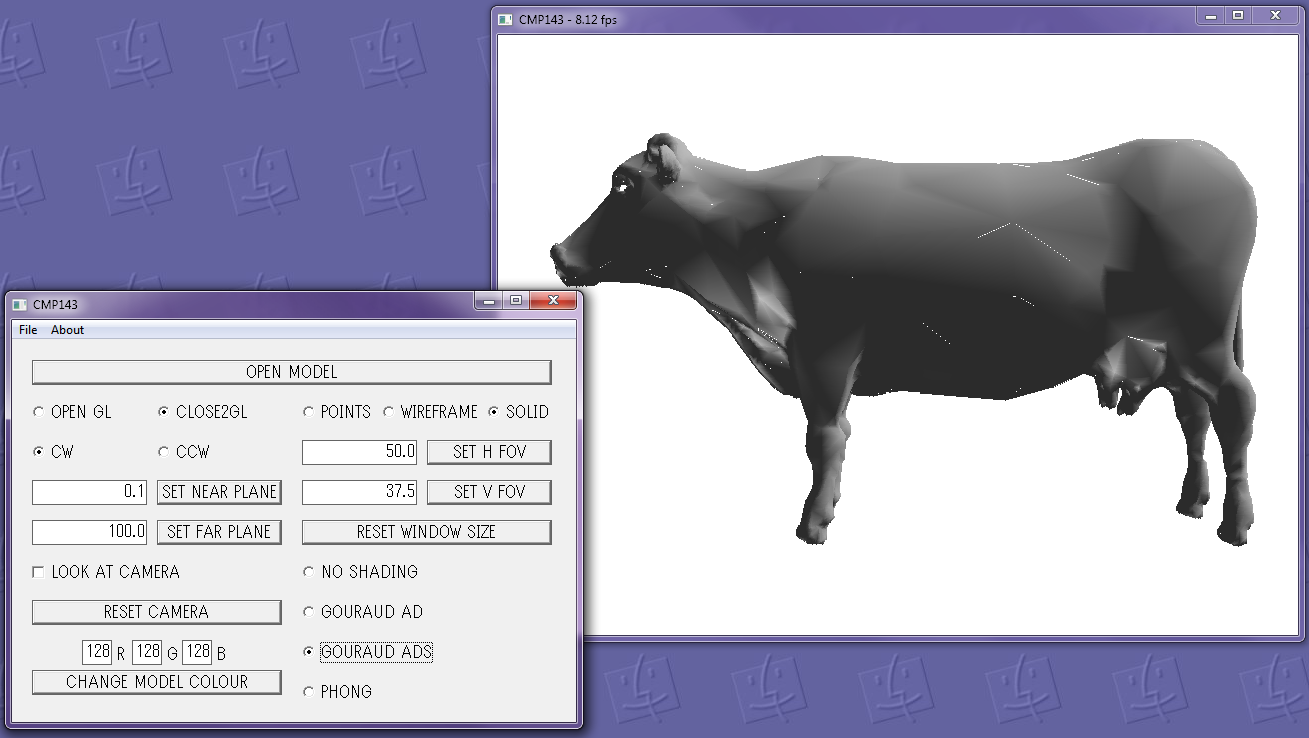
\includegraphics[scale=0.45]{5.png}
\end{center}
\begin{center}
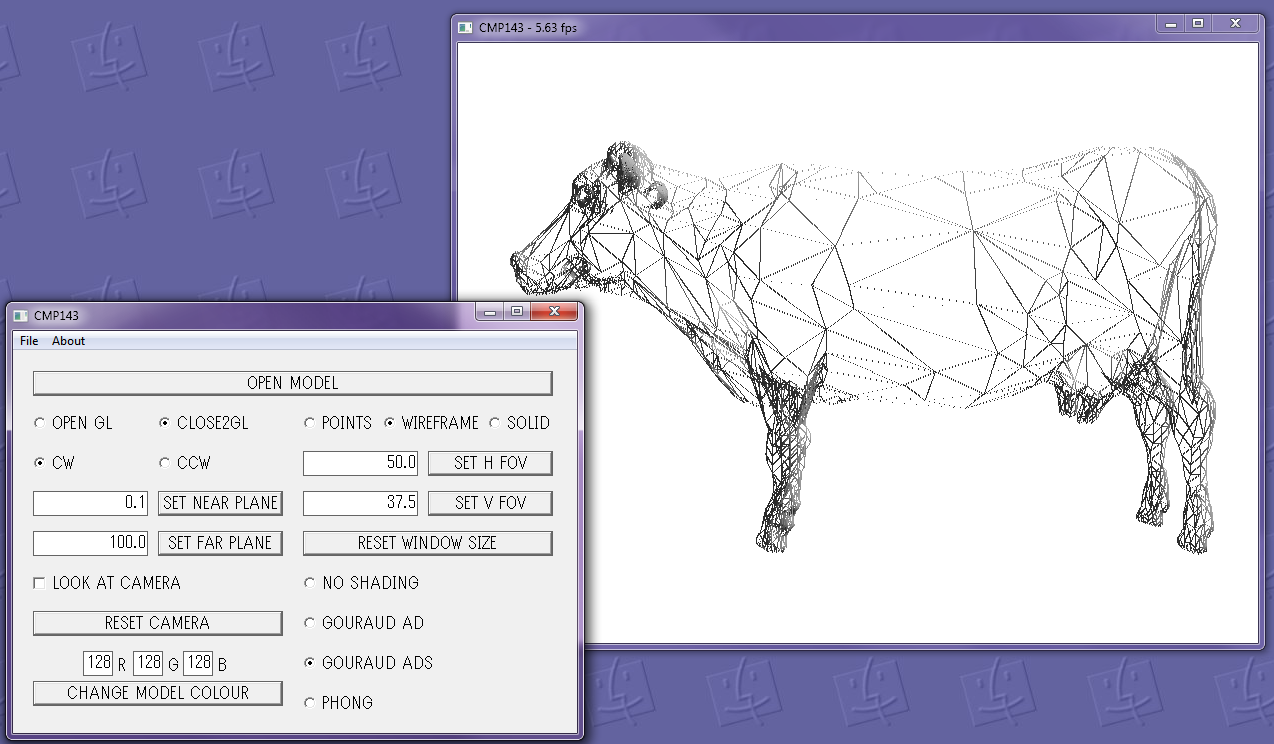
\includegraphics[scale=0.45]{9.png}
\end{center}
These were implemented using Gouraud shading.
\newpage
It works with both clockwise and counterclockwise orientation of the vertices:
\begin{center}
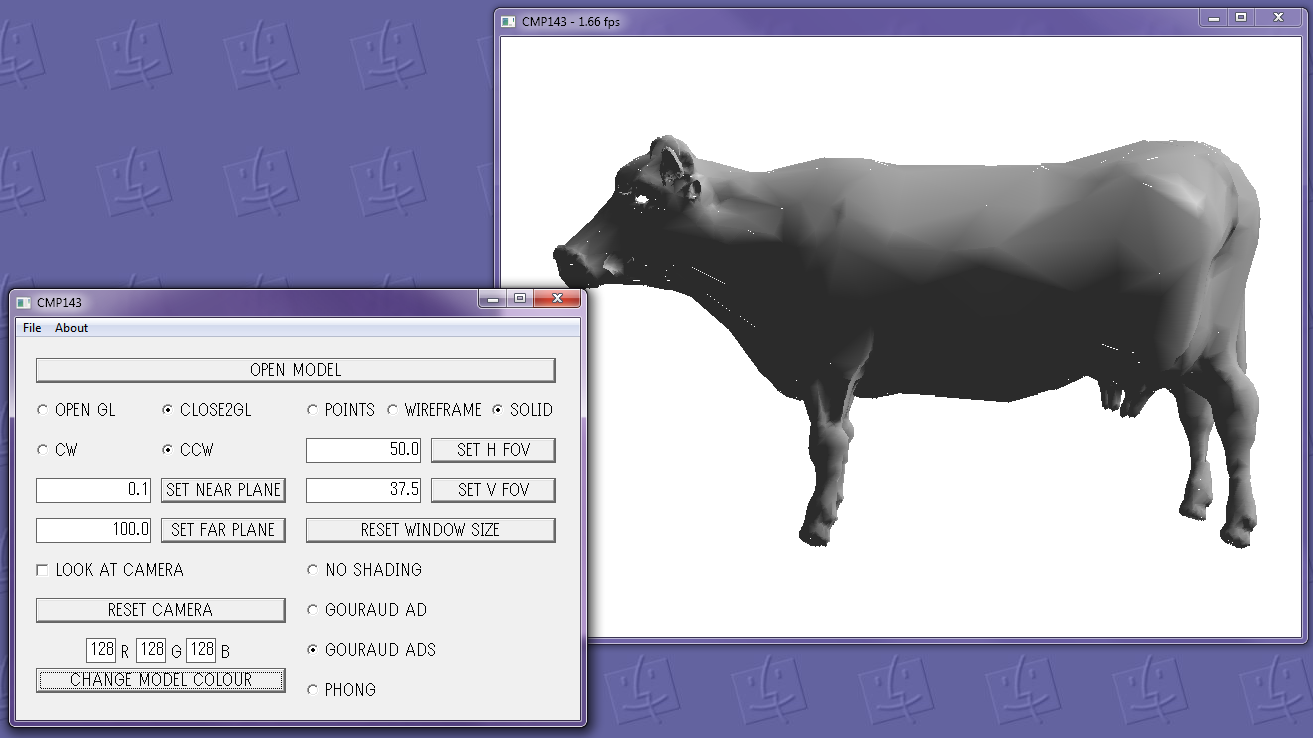
\includegraphics[scale=0.45]{7.png}
\end{center}
And it works if the screen is resized or the color of the model is changed:
\begin{center}
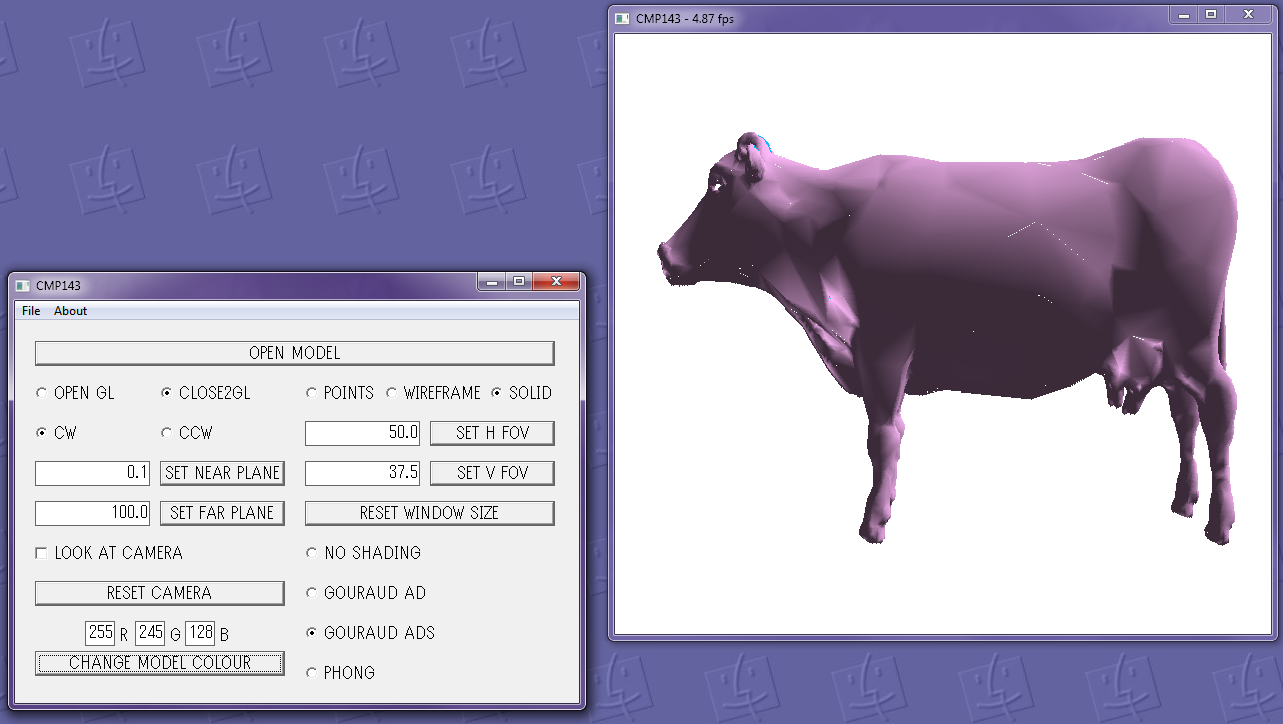
\includegraphics[scale=0.45]{6.png}
\end{center}
\newpage
It also works fine if the camera orientation changes:
\begin{center}
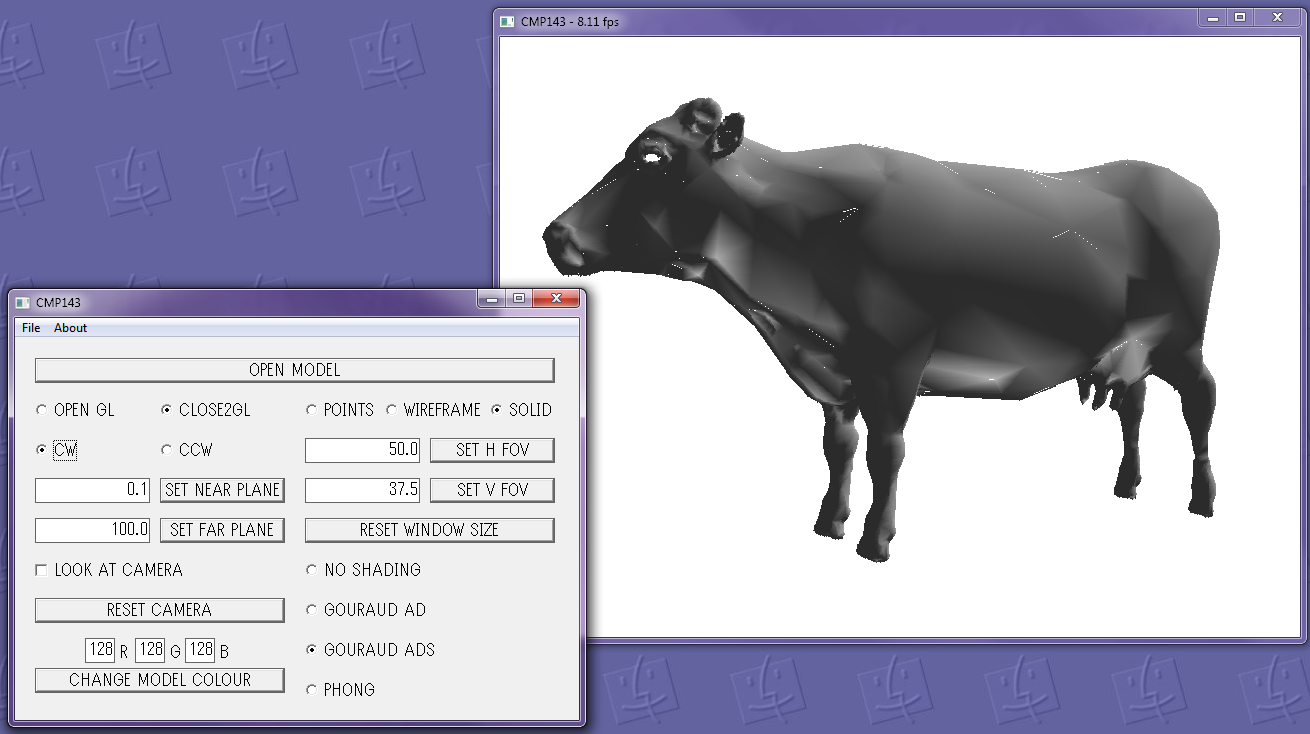
\includegraphics[scale=0.45]{8.png}
\end{center}
\end{document}